\documentclass[../main.tex]{subfiles}
\begin{document}
\begin{figure}
    \centering
    \begin{subfigure}[b]{0.48\textwidth}
    	\centering
	    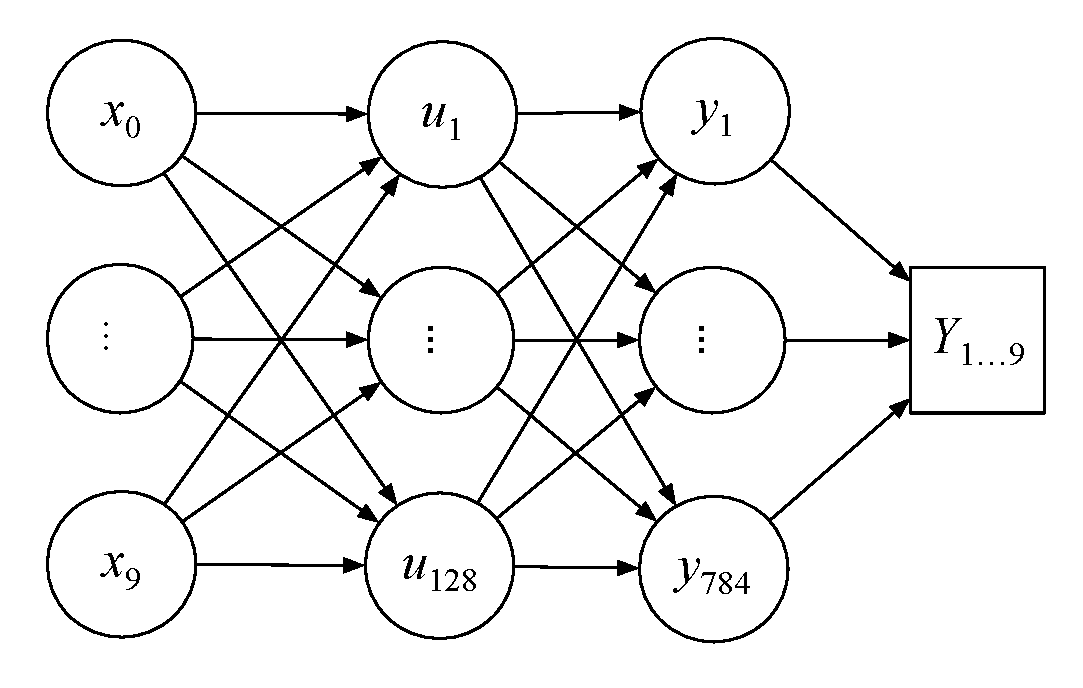
\includegraphics[width=\textwidth]{figures/wgan/generator}
	    \caption{Neural network used for the generator network $\mbf{G}$.}
	    \label{fig:g}
    \end{subfigure}
    ~
    \begin{subfigure}[b]{0.48\textwidth}
    	\centering
	    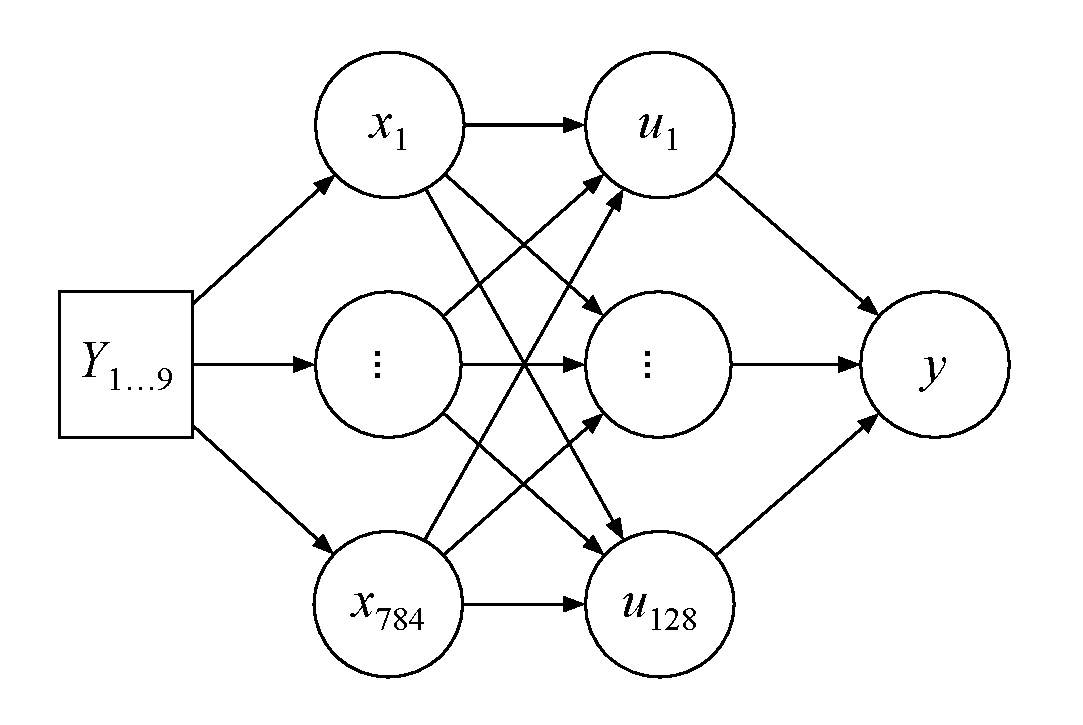
\includegraphics[width=\textwidth]{figures/wgan/discriminator}
	    \caption{Neural network used for the discriminator network $\mbf{D}$.}
	    \label{fig:g}
    \end{subfigure}
    \caption{The Neural network of $\mbf{G}$ and $\mbf{D}$.}
\end{figure}

\begin{figure}
    \centering
    \begin{subfigure}[b]{0.48\textwidth}
    	\centering
	    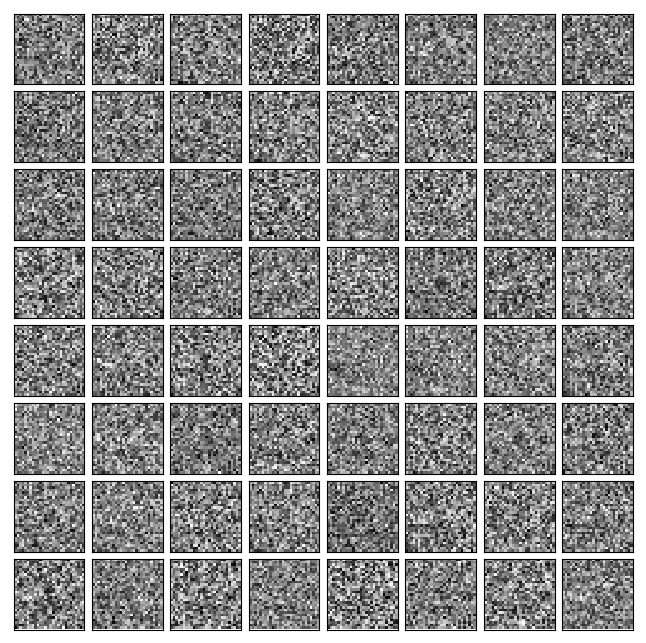
\includegraphics[width=\textwidth]{figures/wgan/0000000000}
	    \caption{The output image of generator network $\mbf{G}$ after 100 epochs.}
	    \label{fig:100epochs}
    \end{subfigure}
    ~
    \begin{subfigure}[b]{0.48\textwidth}
    	\centering
        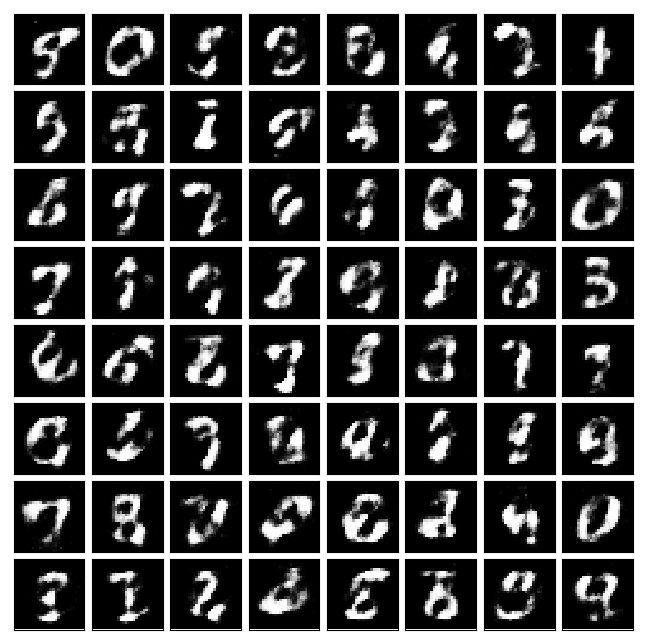
\includegraphics[width=\textwidth]{figures/wgan/0000039000}
        \caption{The output image of the generator network $\mbf{G}$ after 40 000 epochs.}
        \label{fig:lastepochs}
    \end{subfigure}
    \caption{The output of a neural network $\mbf{G}$ that generates digits based on Generative Adversarial Networks.} \label{fig:pix}
\end{figure}

Searches for the previous implementation was used for the generator $\mbf{G}$ and discriminator $\mbf{D}$. We were inspired by the tutorial. We tried with several layers but achieved the best result with two hidden layers. The width of the first hidden layer $\mbf{u}$ was chosen to 128 \cite{tutorial-wgan}. Because the output picture has dimensions of 28 px times 28 px, the last layer $\mbf{y}$ had to be $28^2=784$. The topology of the network \mbf{G} is shown in \autoref{fig:g}. The input $\mbf{x}$ is given so that
\begin{equation}
    \mbf{x}(0)=[1, 0, 0, 0, 0, 0, 0, 0, 0]
\end{equation}
and
\begin{equation}
    \mbf{x}(4)=[0, 0, 0, 0, 1, 0, 0, 0, 0]
\end{equation}
The output $\mbf{Y_{0...9}}$ is a $28\cdot28$  picture that ideally illustrates a number coresponding to $\mbf{x}$. After several trials and errors it was decided to apply different activation functions. There are neither a matrix multiplication nor a bias correction between $\mbf{y}$ and $\mbf{Y}$, only reorganization to a picture. The activation function for $\mbf{u_{G}}$ is ReLU and Sigmoid for $\mbf{y_{G}}$.

The discriminator $\mbf{D}$ is applying the opposite action. It takes a picture $\mbf{Y_{0...9}}$ as an input and then reorganizes it to $\mbf{x}$. It has only one hidden layer $\mbf{u_{D}}$ of width 128. The discriminator $\mbf{D}$ uses the activation function ReLU. 

The discriminator $\mbf{D}$ is trained on the MNIST dataset five times for each time the generator $\mbf{G}$ train against $\mbf{G}$. It's important to use a sufficiently small number of training of $\mbf{D}$ for each time $\mbf{G}$ is trained. If this number is too large, then $\mbf{G}$ will not be able to improve as $\mbf{D}$ will discard all attempts by $\mbf{G}$. The initial learning rate applied was chosen to
\begin{equation}
	\alpha_0 = 1 \cdot 10^{-4}
\end{equation}
The learning rate then decay exponentially so that
\begin{equation}
	\alpha(i)= \alpha_0 \cdot 0.99^{\frac{\rm i}{1000}}
\end{equation}
where $i$ is the epoch index and is increasing by 1 for each iteration. The batch size is 64. The final results for epochs of 100 and 40 000 is shown in \autoref{fig:pix}.

\subsection{Cross-entropy error for $\mbf{G}$ and $\mbf{D}$.}

\begin{figure}[t]
	\centering
    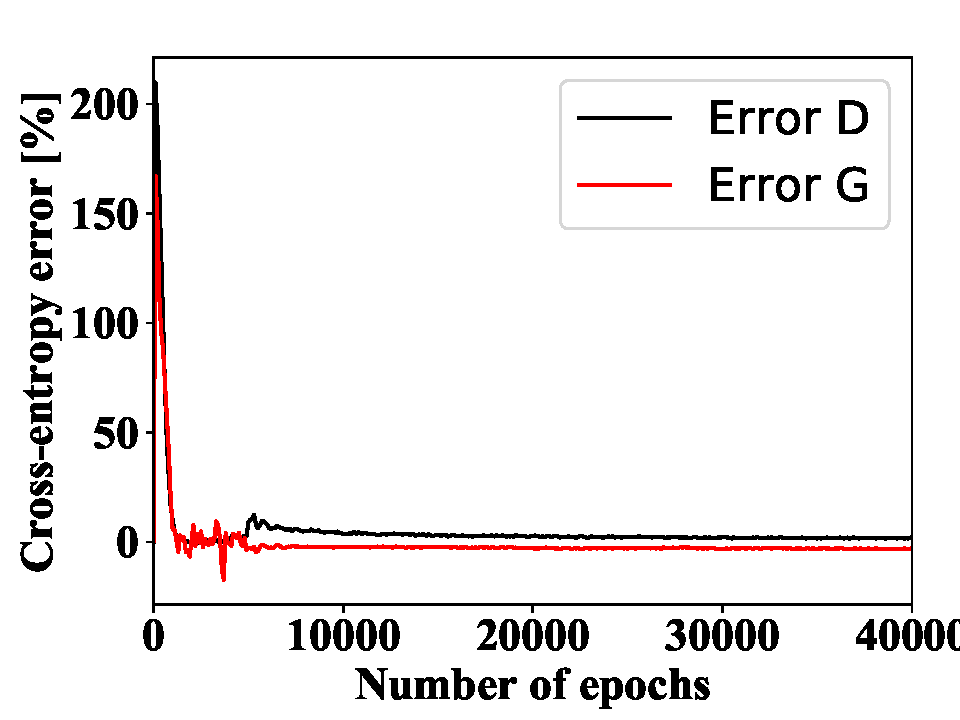
\includegraphics[width=0.48\textwidth]{figures/wgan/cross_entropy_error.pdf}
    \caption{Cross-entropy error of $\mbf{G}$ and $\mbf{D}$.}
    \label{fig:cer3}
\end{figure}

The cross-entropy error function for $\mbf{G}$ is given by
\begin{equation}
	E_{\mbf{G}} = -E_{\rm rm}(\hat y_{f})
\end{equation}
where subscript $f$ indicates the estimated $y$ by $\mbf{D}$ for picture generated by $\mbf{G}$. $f$ is short for fake. The cross-entropy error function for $\mbf{D}$ is
\begin{equation}
	E_{\mbf{D}} = E_{\rm rm}(\hat y_{r}) + E_{\mbf{G}} \label{eq:E_d}
\end{equation}
where $E_{\rm rm}(\cdot)$ is the reduced mean error. Subscript $r$ indicates estimation on real images from the discrimination training set. The cross-entropy errors $E_{\mbf{G}}$ and $E_{\mbf{D}}$ are shown in \autoref{fig:cer3}. The error starts relatively low, as $\mbf{D}$ is not yet well trained in discriminating generated photos. The error then decreases dramatically, as shown below
\begin{lstlisting}[language=Python]
Epoch:  0 lr  0.0001
	 Generator error:	0.0063119
	 Discriminator error:	-0.0009150
Epoch:  100 lr  0.0001
	 Generator error:	1.6718566
	 Discriminator error:	2.0977683
\end{lstlisting}
After the initial rise, the error falls dramatically, as both $\mbf{G}$ and $\mbf{D}$ becomes better. $\mbf{G}$ oscillates around $\mbf{D}$ for a time as shown below
\begin{lstlisting}[language=Python]
Epoch:  200 lr  0.0001
	 Generator error:	1.4765003
	 Discriminator error:	1.9077775
Epoch:  300 lr  0.0001
	 Generator error:	1.1227739
	 Discriminator error:	1.6191332
Epoch:  400 lr  0.0001
	 Generator error:	0.9557722
	 Discriminator error:	1.3049076
\end{lstlisting}
This is because $E_{\mbf{G}}$ is highly dependent on the discrimination capabilities of $\mbf{D}$. Both of the cross-entropy errors $E$ stabilizes around 0. The whole trend is shown in \autoref{fig:cer3}.
\subsection{What type of learning is GAN?}

According to OpenAI, which the authors find as a credible source, the GAN is a unsupervised learning algorithm \cite{openAIBlog}. $\mbf{G}$ is unsupervised as it doesn't get any feedback from real cases, as they does not apply. However, the authors of this report will argue that $\mbf{D}$ is semisuprvised as it gets a boolean value from several real examples yet adjusted by the cross-entropy error of $\mbf{G}$, as shown in \autoref{eq:E_d}. 
\end{document}